% \documentclass[10pt,twocolumn,oneside]{article}
\documentclass[10pt,onecolumn,oneside]{article}
% \usepackage{simpleConference}
\usepackage{times}
\usepackage{graphicx}
\usepackage{colortbl}
\usepackage{todonotes}
\usepackage{url,hyperref}
\usepackage{fancyvrb}
\usepackage{verbatim}
\usepackage[top=1in, bottom=1in, left=1.5in, right=1in]{geometry}
\usepackage{fixltx2e}
% \usepackage[backend=bibtex]{biblatex}

%Remove hyphens
\usepackage[none]{hyphenat}

\begin{document}
\title{System-wide Performance Analysis for Virtualization}
\author{Deron Jensen\\
\\
Department of Computer Science\\
Portland State University\\
Portland, OR \\
deron@cs.pdx.edu \\
}
\date{\today}
% \onecolumn[
% \begin{@twocolumnfalse}
  \maketitle

\begin{abstract}
With the current trend in cloud computing and virtualization, more organizations are moving their systems from a physical host to a virtual server.  Although this can significanlty reduce hardware, power, and administration costs, it can increase cost in analyzing performance problems.  With virtualization, there is an initial performance overhead, and as more virtual machines are added to a physical host the probability of interference between various guest machines running different applications increases.  When this interference occurs, a virtualized guest application may not perform as expected.  Additionally, there is little or no information to the virtual OS about the interference.  From the hypervisor viewpoint, tools are available to view each virtual machine, but the overhead and interference is not available. \newline
\indent  We examine the interference that has been shown in previous research, and relate that to existing tools and research in root cause analysis.  We show that in virtualization there are addtional layers which need to be analyzed, and devise a framework to determine if degredation is occuring from a external virtualization layer.  Additionally, we build a virtualization test suite with Xen and Postgresql and run multiple tests to create I/O interference.  We show how our framework can help determine if the problem is from external interference when an application is degraded.   
  \end{abstract}
% \end{@twocolumnfalse}
% ]

\onecolumn
% 1.  This is a comment
\section{Introduction}
System virtualization is a way for a data center to reduce cost and power by overcommitting and sharing system resources across disparate operating systems with common hardware.  Since each guest machine only uses a portion of the available resources at any given time, the total resources allocated to all guest VMs can exceed the total physical resources \cite{huber2, amit, buell1}.   This idea of overcommitting resources is the same as preemptive multitasking, where multiple processes share a single CPU; and OS virtual memory, where the total memory available to applications exceeds the physical memory capacity.   

\indent Due to these cost savings and lower physical administration overhead, IT Data Centers and Businesses are moving toward virtualized environments.  In 2008 Gartner’s showed that 12\% of hardware at data centers were virtualized, and then predicted that by 2013 61\% would be virtualized \cite{gartners}.   Additionally, research from Ramya and Edwin show tremendous growth in Platform As A Service (PAAS) where an entire system platform is dynamically provisioned in a cloud computing service \cite{ramya}.   Massive data centers are able to provide virtual systems, and manage large clusters of shared resources, while meeting expected Service Level Agreements, for a fraction of the price of building a physical server for each customer.

\begin{figure}[!b]
  \begin{center}
    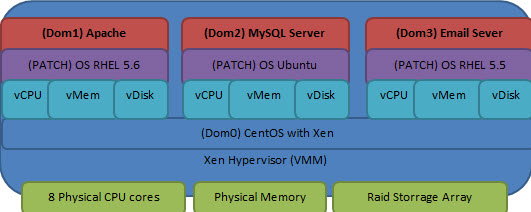
\includegraphics[width=3.5in]{images/VirtualizationExample.jpg}
  \end{center}

  \caption{\small In this example there are 3 paravirtualized guests (DomU) running on a Xen Server.  The Xen hypervisor and Dom0 divide, share, and overcommit the physical resources between the 3 guest domains.  Each guest has access to virtual resources and not physical hardware.}
  \label{fig-VirtualizationExample.pdf}
\end{figure}


\indent The problem this introduces is in performing profiling and analysis of this additional layer of abstraction.  The hypervisor, or Virtual Machine Manager, adds to the already complex existing layers (Application, OS, and Hardware) one must analyze when an application performs sub-optimally.  How can a system administrator determine if the problem is in the application, OS, hypervisor, hardware, or an unrelated guest virtual machine on the same physical host system?  In a traditional environment there can be 'interference' \cite{paul}or ‘system noise' caused by these layers, which attributes to poor application performance.  The hypervisor as well as multiple other guest virtual machines which compete for system resources add to this outside interference, which is undetectable from a guest VM, and therefore undetectable by the guest applications.

\indent This paper we show that using existing profiling tools and measuring changes in system runtime data in the guests and VMM we are now able to determine the layer of the complex software stack that attributes to a sub-optimal running application in a virtual environment.  Additionally, we can determine which system resource (memory, CPU, or IO) needs to be modified or is used inefficiently.

\indent This project will add the following contributions for virtualization:
\begin{enumerate}
\item Define the layers of abstraction in various virtual environments.
\item Define the system resources which attributes to application problem from I/O, memory, or CPU problems.
\item Framework to Identify the counters, metrics, and envirement at each layer which contributes to I/O contention.
\item Example tool which dynamically analyzes runtime interference and identifies the layer which experiences I/O contention.
\item Introduce \emph{disk pinning} for virtualization where separate physical disks are assigned to individual virtual servers.
\end{enumerate}




\section{Motivating Example}
A large US corportation, with over 10,000 employees and 200 franchises had a custom application for a retail business that sold and serviced merchandise.  A suite of applications which had been specifically written for this business consisted of a core inventory, service, accounting, and several other add-on services.  The OS consisted of Redhat based Linux with 2.6.18 kernel, Postgresql 8.3.6, and Apache 2.2.3 The hardware had 40 CPU cores (4 sockets 10 cores each) and 256 GB of RAM with a high end RAID SAN used for the data store.  At most times during the business day the system would run with less than 60\% total CPU and would cache nearly all data inside active RAM.   The system ran optimally for several months in this configuration, and was hosted in a data center.

\indent At some point the customer and data center decided to virtualize the application to add disaster recover and save power.  After several weeks the end users started to complain and enter trouble tickets about slow response times in the web server.  Application developers and support quickly found issues and developed fixes.   Usually these fixes were to reduce the number or reads or writes to some file in the filesystem.  However, after each fix, sometimes days later, a new problem would show up.  Eventually the database engineers and system engineers began examining the recurring problems.

\indent The symptom was that sometimes the system would go into a state where all 32 cores would go to 100\% CPU time, multiple threads would go to a “D state” \footnote{A procees in the D state is neither running nor sleeping.  It is "Uninterruptable sleep (usually IO)"} , and multiple processess would just not complete.   The additional CPU time was shown to be in \emph{System Time} and multiple tools confirmed this.  Memory and IO used on the guest and host server were consistent, and engineers monitoring the SAN did not see any latencies or problems measuring disk IO.  Sometimes this would only last a few seconds and sometimes it would last for hours. At some points the \emph{strace} output of Apache process would hang for several seconds on system calls to \emph{open}, \emph{lseek}, and \emph{write}.  See Figure \ref{fig:syscalls} for details.

\begin{figure}
%\begin{Verbatim}[frame=single]
\begin{Verbatim}
12:46:02 open("…", O_WRONLY|O_CREAT|O_
12:46:16 fstat64(61, {st_mode=S_IFREG| 
12:46:16 lseek(61, 0, SEEK_CUR) = 0 
12:46:24 write(61, "O:6_"..., 8192) =  
12:46:24 write(61, "R1339 "..., 8192)  
12:46:24 write(61, "ct "..., 8192) = 8 
12:46:31 write(61, "cription "..., 819  
12:46:31 write(61, ";s:11 "..., 8192)  
12:46:31 write(61, "7:for "..., 3288)  
12:46:31 close(61) = 0
\end{Verbatim}
\label{fig:syscalls}
\caption{\emph{strace} shows system calls to open, lseek, and write take up to 14 seconds to complete}
\end{figure}

\indent Looking at statistics in the VMM showed exactly what was noticed on the guest.  High CPU usage, but from the point of view of the VMM, there was no difference between guest time and kernel time and appeared as though there was a misbehaving guest application or guest kernel.  However, no symptoms appeared until the application was virtualized.  The guest was unable to perform profiling with hardware coutners on this version of the hypervisor \cite{serebrin} to see if there was a kernel bug.  Was there a bug or misconfiguration in the application, guest OS, hypervisor, or hardware?  Or was there just too much overhead from virtualization during peak usage?


\section{Virtualization and Profiling}
\subsection{Profiling}
Profiling allows a user or system administrator to see which functions are being called the most frequently or consume the most time.  Oprofile \cite{levon} is a profiler that can profile both application and kernel functions, by registering with the Performance Monitoring Unit (PMU) on the CPU.  The PMU will track hardware counters and will notify the registered profiler when a specific hardware counter reaches a threshold set by the profiler \cite{mucci}.  When Oprofile receives notification, through an NMI, it will record the PC and other information about the system, and over time will have the most frequently called function when the specified hardware event occurred.  Some typical hardware event counters are:  TLB miss, LLC cache miss, or CPU instructions retired.   Other profilers like OSprof use latency distribution analysis [7].  As function calls are entered and exited to or from the stack, the profiler tracks the start and end time of the functions.

Research at VMware \cite{serebrin} shows the importance and challenges of implementing hardware counters on the PMU for analyzing interference from a virtual guest perspective.
The difficulties with running a profiler like Oprofile in a virtualized guest is that the hardware counters in the guest may not be available for all hypervisors \cite{buell1}.  Additionally, the guest is not guaranteed to receive interrupts in a correct order.   Tracking the wall-clock time and CPU time on virtual machines is extremely difficult and there are many additions in the hypervisor to help guest machines accurately track time.  On many systems, kernel level profiling is not enabled. A patch or configuration change is needed to enable profiling, which makes it difficult on production systems.
In the Xen environment, Xenoprof allows the virtual guest to read hardware performance counters from the guest OS perspective \cite{menon, du2}.  However, Xenoprof does not analyze the results or draw any conclusions about the counters.  

\indent In virtualization there are 2 types of profiling:  Guest-wide profilers only profile a single guest (or domain), and System-wide which monitors all guests and the VMM \cite{du1}.  In order to provide Guest-wide profiling for virtual systems, the profiler runs in the guest and the VMM needs to provide synchronous delivery of interrupts from the hardware to the guest machines.  For System-wide profiling the profiler runs in the VMM and requires interaction between the guest OS and VMM.  Specifically, the VMM needs to know which application and kernel functions are running on the guest machine at the time of the interrupt.

\indent Xenoprof uses Oprofile to provide the profiling and uses Xen's hypercalls to share information between the guest and Xen Hypervisor.  The Xenoprof toolkit supports system-wide coordinated profiling in a Xen environment.  The underlying Oprofile uses statistical profiling across domains and can track functions running in the user space, kernel space, and in the hypervisor.  Xenoprof provides a performance event interface which maps physical hardware events to virtual HW counters \cite{santos, menon2}.   The guest-level profiling registers with the virtual CPU, and the hypervisor registers with the physical hardware.  Since it is not possible to call the domain level virtual interrupt handler synchronously, Xenoprof collects the samples for the guest domain and logs them to that specific domain buffer, and then Xenoprof sends a virtual interrupt to the guest domain.

\indent In KVM, a Linux Kernel VM subsystem, a customized profiler can implement both guest-wide and system-wide profiling \cite{du2}.  Linux perf is another profiler that runs in the Host Linux on KVM, and can measure software and hardware event counters as well as tracing.  It is aware of the memory layout of the guest and can monitor the Kernel space of the guest VM, but not its user-space application. 

\begin{comment}
\indent VMware ESX sever strives to provide a complete full virtualization including hardware counters to allow any guest profiling to work as if it were on native hardware.  VMware creates a virtual timer for the guest OS, but the profiler may need relative time difference and track only time on the Virtual CPU.  Additionally, there needs to be a way to efficiently and accurately emulate interrupt events from the virtual machine to the host. These techniques are classified as speculative and non-speculative events, and the Hypervisor may try to give the guest a complete view of system in order to run any Profiler in the unmodified guest OS.  VMware provides VMKperf in order to profile the hypervisor, but does not profile the guest OS.
\end{comment}

\indent Profiling results also require manual inspection and may not show how interference from external layers impact the guest machine \cite{traeger, knapp1}.  Additionally, the user running the profiler needs to have some "guess" or prior knowledge about what event to sample, and the desired frequency of the sample.  Should the user sample cache miss, TLB miss, or some other counter?  As more events are profiled, the more perturbation is encountered.  In a virtual environment a user may need to start several profilers on several virtual machines each monitoring various hardware counters, system state, and applications.  Only after several runs in many different configurations and manual inspection could an advanced administrator make some determination as to the root cause of the problem. 

\subsection{Performance Monitoring}
Modern operating systems have a method of monitoring the current performance of the system.  User tools use statistics tracked in the kernel to monitor access to resources, and are not (necessarily) related to the PMU on the CPU.  For example a specific CPU may track hardware events such as L2 cache miss, or TLB cache miss, but the kernel will track time spent reading or writing to a physical disk, or virtual memory cache information.  User tools aggregate and relate these statistics to provide the user some inference about the system.

\indent In a Linux OS there are administration tools such as top, iostat, ps, and vmstat.  
Windows uses \emph{Performance Monitor} or \emph{Resource Monitor} to show the current performance.  
Most kernels will write statistics when each resource is used, and these tools read and analyze the kernel data about resource usage, through the method provided by the kernel.
By examining these counters and aggregating the data with tools, an administrator can see the current threads and how each of the resources are being used. 

\indent When a system is virtualized, the guest OS kernel only tracks the statistics from its own viewpoint.  
In other words, the resource statistics are for the virtualized resource, and not the physical resource.   
The counters do not collect information from external guests or show the interference from external guests or the hypervisor.  
The host system kernel will track all the guests, but is unable to identify which process in the guest may be degraded.
In order to accurately analyze performance issues on complex virtualized systems, we need to collect and analyze resource usage from all systems and the hypervisor.  
We need the ability to perform System-wide performance monitoring similar to the System-wide profiling available.

\subsubsection{Linux Tools}
\indent On Linux the kernel resource counters are tracked in the /proc file system, which is a dynamic view into the kernel data structures and statistics \cite{proc}.  
For example \emph{/proc/stat} contains statistics about the time (since boot) that the the CPU was idle, running in user mode, or running in kernel mode.
By running a test load and examining the /proc file system, one can reasonably determine the resources used and which process or thread is using them.  
Without virtualization, these tools can quickly narrow the scope of possible problems for a degraded system. 

\begin{figure}[h]
\begingroup
    \fontsize{10pt}{12pt}\selectfont
\begin{Verbatim}
top - 15:57:05 up 109 days, 23:54,  6 users,  load average: 0.12, 0.17, 0.11
Tasks: 164 total,   1 running, 163 sleeping,   0 stopped,   0 zombie
Cpu(s):  6.0%us,  0.7%sy,  0.0%ni, 93.3%id,  0.0%wa,  0.0%hi,  0.0%si,  0.0%st
Mem:   2062348k total,  1868648k used,   193700k free,   185776k buffers
Swap:  2095100k total,   389996k used,  1705104k free,   699236k cached

  PID USER      PR  NI  VIRT  RES  SHR S %CPU %MEM    TIME+  COMMAND            
  999 root      20   0 94876  52m 4900 S  4.0  2.6 373:01.16 Xorg               
 5362 deron     20   0  317m  92m  62m S  2.0  4.6 300:20.40 soffice.bin        
25333 deron     20   0  140m  15m 5684 S  1.0  0.8   3:33.53 gnome-terminal     
 1859 deron     20   0  166m 5820 4028 S  0.3  0.3   3:15.13 metacity           
\end{Verbatim}
\endgroup

\caption{\emph{top} collects information from Linux kernel through \emph{proc} and displays information about CPU, Memory, and processes}
\label{fig:top}
\end{figure}

\subsubsection{Windows Tools}
On Windows OS the counters are similar and are tracked by the Windows kernel about processes and threads.  The user space API \cite{winperf} is used by the user application to display graph or report. The GUI administration tool can display any number of statistics about the system.  Similar to the /proc file system in Linux there is little or no information provided about the overhead and interference from external layers.

\begin{figure}[!h]
  \begin{center}
  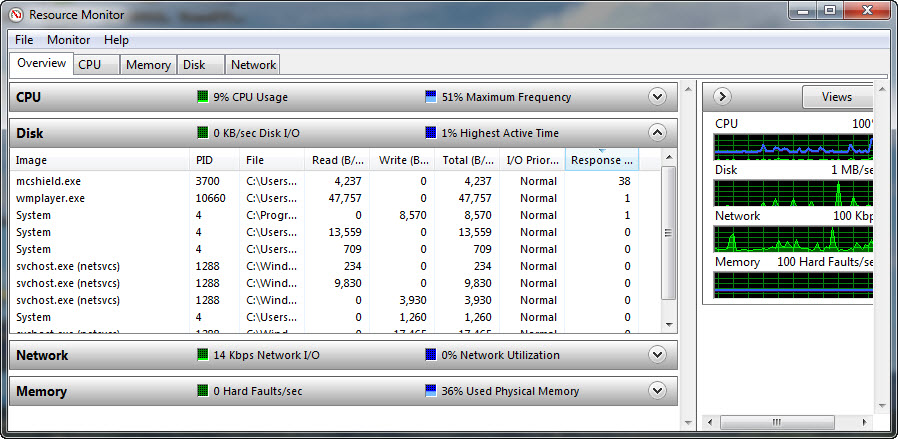
\includegraphics[width=6in]{images/ResourceMonitor.jpg}
  \caption{Microsoft Windows Resource Monitor.  Reads data from Winperf API tracked in Windows kernel}
  \label{resourceMonitor}
  \end{center}
\end{figure}

\subsubsection{Hypervisor Tools}
Similar tools have been created in the hypervisor, \emph{xentop} for Xen and \emph{esxtop} for VMware, to show each virtual machine running and the resources that the entire machine is using.  
These tools use the same information from the \emph{proc} file system as VMware and Xen use a Linux based kernel.  
From this view we can see the guest machines, and the hypervisor, but we can't easily determine how they impact each other.  There is also no way to relate a virtual process running in the guest machine from the hypervisor tools.  The hypervisor has no access to the guest information.
Even if the these could show everything running in the guest machines, the administrator for the hypervisor and guest machines are different people or even completely different organizations. 

\begin{figure}[h]
\begingroup
    \fontsize{10pt}{12pt}\selectfont
\begin{Verbatim}

xentop - 17:07:00   Xen 4.2.2-23.el6
5 domains: 3 running, 2 blocked, 0 paused, 0 crashed, 0 dying, 0 shutdown
Mem: 4182752k total, 4182236k used, 516k free    CPUs: 4 @ 2133MHz
      NAME  STATE   CPU(sec) CPU(%)     MEM(k) MEM(%)  MAXMEM(k) MAXMEM(%) 
  Domain-0 -----r      78969   16.9    2035712   48.7    2097152      50.1    
  Test_VM1 -----r       6474   11.5     524288   12.5     524288      12.5     
  Test_VM2 -----r       4642   12.7     524288   12.5     524288      12.5 
  Test_VM3 --b---       4210    0.1     524288   12.5     524288      12.5     
  Test_VM4 --b---       4137    0.1     524288   12.5     524288      12.5  
\end{Verbatim}
\endgroup
\caption{\emph{xentop} 4 Guest domains. Hypervisor does not get information about guest applications.}
\label{fig:xentop}
\end{figure}

\subsubsection{Steal Time - Complete View}
Due to the fact that the hypervisor has one view of the system, and the virtualized guests have a different view of the system, the Xen Hypervisor has added a \emph{steal time} statistic and made it available to the guest operating systems.  New Linux distributions have implemented this new kernel option as \emph{steal: involuntary wait} \cite{proc}.  Additionally, administrative tools top, sar, and vmstat have all implemented this new counter.  
On most systems top will show as '0.0\%st' (Figure ~\ref{fig:top}), but if it is running on a Xen Hypervisor the paravirtualized guest will communicate with the hypervisor and collect information. Amazon cloud uses Xen and this has become a valuable tool for guests to determine if they are having performance problems from external interference \cite{netflix}.



\section{Related Work}
Several papers have been written to try to analyze, quantify, or predict application performance when moving from a physical system to a virtual system.   Cherkesova (et. al) show that they can measure and quantify the CPU overhead for moving from a physical to virtual machine.  Additionally they formulate a method for “charging” a machine for excessive I/O which ends up causing CPU contention on an unrelated VM \cite{cherkasova}  Research at VMware also show this contention, and formulate that it is due to additional Inter Processor Interrupts (IPI) \cite{ahmad}.   This contention is more prevalent to the virtual environment, because the guest may run on one CPU, and the hypervisor will run on a separate CPU.  
\indent Disk and network I/O is a major problem when running multiple guests with I/O intensive applications such as file servers and database servers.  Research at Georgia Tech \cite{paul} analyzes the impact of combinations of I/O, CPU, and memory intensive applications running in various combinations.  They conclude that when a File Server and DB Server are placed together they result in a 25\% - 65\% degradation.  This is in contrast to CPU application research \cite{huber1, huber2} which can be allocated per VM (CPU core pinning) and will operate with about 5\% overhead.  Additionally they show that CPU intensive applications can scale at a rate near optimal 1/x.   For Example, if 4 CPU intensive applications running at rate x on 4 fully loaded cores, then they will all run at about 1/4 capacity if placed on the same core.   Disk I/O and memory intensive applications do not scale in this manner, because of both visible and invisible interference \cite{ticktoo}.

\indent Ultimately, the goal of this type of research is to be able to automatically know a priori how a virtual machine will run in a given environment.  Recently, researchers at Florida International attempted to predict performance in a virtual environment through several performance models \cite{kunda}.  Through online and offline modeling, and training data, they are able to predict with about a 20\% error rate through various linear regression models.  They also use an artificial neural network statistical model which was able to predict at under 6\% median error rate.   However, in order to predict this performance, the application load rate would need to remain constant.   Additionally, research from Tiketekar (et. al) at Oak Ridge National Laboratory show that it is extremely difficult to generalize a work load \cite{tikotekar}.  They show that similar HPC application benchmarks, which are both CPU bound, can have significantly different results when paired with other applications.  They stress the fact that performance isolation is extremely difficult.

\indent There has been research to find a \emph{root cause} of application degradation which could identify the layer of the problem in traditional \cite{traeger} and high-performance \cite{knapp1} systems.  It has been shown that analysis needs to be competed from a full \emph{end-to-end} perspective of the system \cite{saltzer, gupta1}.  However, most of the research for virtual systems have been on enabling profiling tools, measuring overhead, and detecting interference.  There is still much work needed in analyzing and finding the \emph{root cause} of problems in a virtualized environment.


\section{Design}
Since the system workload, and available resources will continually change, and it is difficult to predict a constant workload across multiple virtual systems, data centers will need the ability to profile and analyze virtual environments.  Application and system profiling tools are available but require manual analysis of the data and possibly detailed knowledge above that of a traditional system administrator, in order to arrive at a probable conclusion.   

\indent Prior to Xenoprof, it was not possible to read hardware performance counters from the guest OS perspective \cite{menon, du2}.  However, Xenoprof does not analyze the results or draw any conclusions about the counters.  For example, in \cite{tickoo} it is shown that there are 'invisible' resources such as the shared LLC cache, and show that scheduling CPU intensive VMs on the same socket but different cores will result in significant degradation.  Conversely an I/O intensive application with a CPU intensive application on the same configuration will run with little interference.  Where if this I/O and CPU load runs on the same CPU the I/O intensive application will perform optimally, but will significantly degrade the CPU intensive application due to multiple interrupts to read the data from the virtual controller.

\indent This project will add the following contributions for virtualization:
\begin{enumerate}
\item Define the layers of abstraction in various virtual environments.
\item Define the system resources which attributes to application problem from I/O, memory, or CPU problems.
\item Identify the counters, metrics, and envirement at each layer which contributes to I/O contention.
\item Dynamically analyze runtime interference and identify layer for database applications which experiences I/O contention at different layers.
\item Introduce \emph{disk pinning} similar to core pinning (assigning a guest OS to a specific core), where separate physical disks are assigned to individual virtual servers under a constant load.  
\end{enumerate}

\subsection{Abstraction Layers}
In order to find the cause of a problem application, the first step needs to isolate the problem to a specific layer.  If an application is degraded, it could be a problem with the applicaiton, OS, or hardware.  In a virtual environment, the hypervisor also needs to be considered as a cause of the problem.  
\newline
\begin{tabular}{ l p{5cm} }
  layer & definition \\
  \hline
  Application & Includes all code running in user space on a guest machine, inluding the system runtime libraries. \\
  OS & Includes all kernel code and device drivers. \\
  Virtual Guest & An external virtual system. \\
  Hypervisor & The hypervisor and VMM to manage the guest domains. \\
  Hardare & Physical hardware. \\
\end{tabular}

\subsection{Physical and Virtual Resources}
In order to determine the actual cause of the performance problem the next step is to identify the resource which is the most influential to the performance problem.  If the problem is in the Guest OS, then the resource would be a virtual resource.  The goal is to determine if the application is bound by Memory, I/O, or CPU.  In other words, adding \emph{additional} either Memory, I/O, or CPU would improve application performance.  
\newline

\begin{tabular}{ l p{5cm} }
  Resource & Definition \\
  \hline
  Disk I/O & The application is spending more time than normal for Disk I/O. \\
  Network I/O & The application is spending more time than normal for Network I/O. \\
  CPU & The application is spending excessive time computing. \\
  Memory & The application is requesting more memory or requires additional swappping. \\
\end{tabular}

\newline 
The following tools are available to collect data:
\begin{tabular}{ l l p{5cm} }
  Resource & Tool & Description \\
  \hline
  Disk I/O & sar -d & Shows the time the disk was busy, reads and writes per second, wait queue, and service time(seek time). \\
  Uniform Memory & vmstat -a & Active and Inactive page statistics \\
  Uniform Memory & vmstat -s & Virtual Memory table \\
  NUMA Memory & zoneinfo & /proc/zoneinfo \\
  CPU & ps -o <FMT> & Real, system, and clock time \\
\end{tabular}

\begin{comment}
       To see every process with a user-defined format:
          ps -eo pid,tid,class,rtprio,ni,pri,psr,pcpu,stat,wchan:14,comm
          ps axo stat,euid,ruid,tty,tpgid,sess,pgrp,ppid,pid,pcpu,comm
          ps -eo pid,tt,user,fname,tmout,f,wchan

PROCESS STATE CODES
       Here are the different values that the s, stat and state output
       specifiers (header "STAT" or "S") will display to describe the state of
       a process:
       D    uninterruptible sleep (usually IO)
       R    running or runnable (on run queue)
       S    interruptible sleep (waiting for an event to complete)
       T    stopped, either by a job control signal or because it is being
            traced.
       W    paging (not valid since the 2.6.xx kernel)
       X    dead (should never be seen)
       Z    defunct ("zombie") process, terminated but not reaped by its
            parent.
      For BSD formats and when the stat keyword is used, additional
       characters may be displayed:
       <    high-priority (not nice to other users)
       N    low-priority (nice to other users)
       L    has pages locked into memory (for real-time and custom IO)
       s    is a session leader
       l    is multi-threaded (using CLONE_THREAD, like NPTL pthreads do)
       +    is in the foreground process group.
\end{comment}

\subsection{Detecting I/O Interference}
It has been demonstrated that I/O is a major contributor to significant degradation in a virtual enviroment.  Normally, the goal of the OS is to delay, cache, and merge physical I/O requests.  However, if the \emph{working set} for a heavy I/O application like a database exceeds the available memory of the application, the application becomes I/O bound and caching in memory becomes less effective.
At each layer data and statistics need to be collected to determine why the application may be degraded.
\newline

\begin{tabular}{ l p{5cm} }
  Layer & Counter \\
  \hline
  Application & BytesRead/s BytesWritten/s. \\
  OS & sar virtual I/O and Paging. \\
  Virtual Guest & Hypervisor moitors other guests \\
  Hypervisor & sar physical I/O and Paging. \\
  Hardare & Physical hardware measures IOPS. \\
\end{tabular}

\indent At each layer the analysis tool will need to create a baseline of statistics to track performance counters at various intervals.

\subsection{Disk Pinning}
Disk pinning may be a substitute for multiple I/O bound guest appliations running in a virtual system.  Several papers have demonstrated the effects of core pinning or \emph{core affinity} for CPU bound applications.  This can reduce the load on the hypervisor scheduler and prevent cache contention.  Similarly a single I/O bound guest may use a single disk excessivley causing performance problems on external guests.  RAID systems have been used to improve performance for database applications.  By increasing the number of physical spindles, multiple random disk seeks can occur concurrently.  By setting physical disks to specific virtual guests, we can reduce I/O interference from multiple guests.


\section{Test Suite for IO virtualization}
In order to test our design, two virtualization stacks, a test infrastructure, and several benchmarks were created.  Our test suite runs a load on the guest machines and coordinates the stop and start of the collection of multiple performance counters across the guests and hypervisor.     
Our experiments, when run in this infrastructure, demonstrate the performance problems guest machines may experience, from external interference or changes to the workload.  The performance data collected from all layers of the virtualization stack can distinguish between these different perromance problems.  We run the benchmark at least three times and average the results.

Both virtualization platforms have the same software stack installed (Figure \ref{softStack}).  
We use the Xen hypervisor and CentOS release for both the guest (DomU) and VMM (Dom0).  
This software stack can be extended to mulptiple servers to produce a larger cluster of servers.  
We chose Postgres as the database server for our tests because of its robustness and standard use in hosting facilities and applications.  
It is a good general purpose application that can be used to stress I/O, memory, and CPU resources, although we focused our test suite to measure database read operations.

The test suite can run in all sizes of virtualization environments (Table \ref{virtSize}).  
Tests which run in a \emph{Personal} or \emph{Business} virtualization platform can also be run in a \emph{Cluster} or \emph{Cloud} based system by increasing the size of the database or number of guest machines until a similar load is reached.  
For our experiments we run on an IBM x3650 \emph{Personal} and Dell T410 \emph{Business} sized virtualization environments. 

\begin{table}[h]
\begin{subtable}[h]{0.45\textwidth}
\begin{tabular}{ l p{5cm} }
  Software & Version \\
  \hline
  Hyperviser & Xen 4.2 \\
  Domain 0 & CentOS 6.2 (Kernel 3.4) \\
  Guest Domains & CentOS 6.2 (Kernel 2.6.39) PostgreSQL 8.4 \\
  \hline
\end{tabular}
\caption{Software installed virtualization test stack}
\label{softStack}
\end{subtable}
\hfill
\begin{subtable}[h]{0.45\textwidth}
\begin{tabular}{ l p{5cm} }
  Size & Specifications \\
  \hline
  Personal & IBM x3650 Quad Core 2GB Ram \\
  Business & Dell PowerEdge T410 dual quadcore Xeon processors, 8GB Ram. \\
  Cluster & Multiple small or medium servers clustered together with shared SAN data store. \\
  Cloud & Amazon Cloud or similar PAAS provider. \\
  \hline
\end{tabular}
\caption{Virtualization sizes for tests}
\label{virtSize}
\end{subtable}
\caption{Software and Hardware stacks}
\end{table}

The test infrasture generates a consistent and reproducible system load by using a PostgreSQL database server with PGbench.  
 PGbench creates a TPC-B similar style workload and calculates transactions per second (TPS), so we can track the performance of each guest system from the application layer \cite{pgTune}.  
 We use PGbench to both generate a load to measure overhead and create interference.  
 We can change the database size and the number of users that connect to the database to change the I/O workload from the guest perspective.
PGbench will put a stress load on the limits of the system, and it is a good tool for simulating guest machines that are all consuming as much resources as possible.  
 We measure the TPS from the benchmark when run as a single virtual machine and when run with multiple machines concurrently.  We compare the degradation from the application to our proposed calculation for interference.

When the test runs, each guest VM starts a process which waits for the hypervisor to signal the start of the test.  
 The Dom-0 (VMM) then starts a process which signals all the guests to start, and which benchmark to run.  
 Each guest then collects the $pre$ resource counters and begins running the specified benchmark system load.  
 The domain 0 also collects the same resource counters from its view, but does not generate a load, since in Xen all disk I/O goes through Dom-0, we use this as the hypervisor view  
 When each guest completes the benchmark, it reads the $post$ counters and sends the difference between the two counters back to Dom-0 (Figure \ref{alg1}).
 When the hypervisor has collected the information from all guests, it can display the counters for itself and each guest.
 Executing this once with a single virtual machine, and once with multiple virtual machines we can calculate the interference.

One of the challenges of this test suite is the coordination of the starting and stopping of the test, collection of resource counters, and the information sharing between the guests and hypervisor.  
Since we use Xen as our virtualization platform, we chose XenBus and XenStore \cite{xenbus} to both coordinate the stop and start of the benchmark, and the collection of data results between domains.
In order for paravitualized guest domains to communicate with the hypervisor the XenStore tools for DomU domains had to be built as this is not currently part of the standard package of guest tools.  Other options were to use the TCP/IP stack to send and receive messages between the domains to coordinate the tests and information as well.

For I/O intensive workloads, the application tends to perform very well when the entire \emph{working set} can fit into main memory, and the OS will cache reads from disk.
However, when the \emph{working set}  approaches (or exceeds) the size of main memory, the application tends to degrade quickly.  
Our initial experiments to find an I/O workload highlight this fact by changing the database size under load in a virtual environment.
Before running the entire test suite we need to create a test database that will exceed the \emph{working set} and increase the probability that a database read will need to fetch the data from disk storage.  With PGbench the "-i" flag \emph{scaling factor} is used to initialize a database at a specified size (prior to running the benchmark) so that our results can show changes between a memory bound system and I/O bound system.  

We created a program to find the size of database that would generate a high I/O rate.  It creates a small database then runs a benchmark and collects the results of the benchmark in TPS.  Then it creates a slighly larger database and runs the benchmark again.  This process is repeated until the TPS drop significantly, and the CPU time is almost idle in a I/O wait state.  At this point we can determine an adequate database size for an I/O bound system.

\begin{figure}[!h]
  \begin{center}
  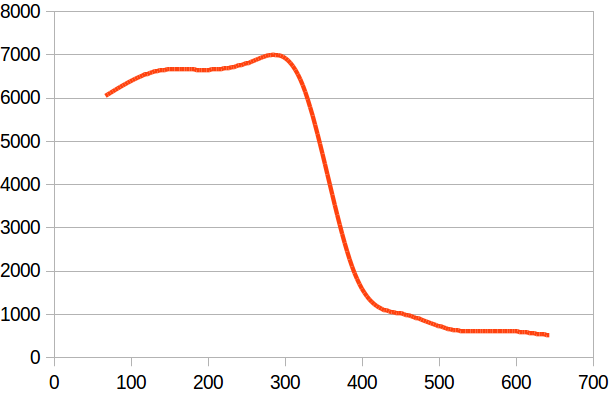
\includegraphics[width=4in]{images/SmallScale.png}
  \caption{TPS on our IBM x3650 system with 1 vCPU and 512KB vRAM. It changes from a memory bound application to an I/O bound application when the DB size approache the available RAM.}
  \label{smallIO}
  \end{center}
\end{figure}

We can use the TPS to show how the database performs at the application layer when external environment changes are made to the system.  Our tests will select Memory and I/O resources to monitor.  For measuring disk I/O it is a good to also collect virtual memory (in this case we are talking about OS virtual memory, not virtualization) as well as I/O data.  We selected to measure paging performance counters \ref{fig:memory} across all layers for the memory resource.  We selected disk read counters \ref{fig:io} as our data at all layers to measure interference from I/O. 



\section{Experimental Results}
In the following test experiments we evaluate the benefits of passing additional information through the layers of the hypervisor and guests for profiling.  Unless otherwise noted, each experiment is performed on a \emph{Personal} and \emph{Business} scale virtualization platform (Table \ref{virtSize}).  Both systems have CentOS and Xen Server installed (Table \ref{softStack}) for the software stack installed.

\subsection{External machine interference}
In this experiment, we show the memory and I/O interference from external systems, without overcommitting the resources.  From the guest domain running the benchmark, there is a significant drop in the application performance when run concurrently with external systems.  Additionally, monitoring resources in the guest domain provides little information about the performance problems. 

First we divide the physical memory and CPUs into four equal parts and create four individual guest virtual machines (Dom1 - Dom4).  Each virtual machine is given 25\% of the availble resources so that no guest virtual machine would interfere with another machine if they were on separate physical systems.  We start only our Dom1 machine and run our experimental test with PGbench.  On our \emph{Business} Dell server, Dom1 is allocated 2GB vRAM and 2 vCPU, while on the IBM server is Dom1 is given 512MB vRAM and 1 vCPU.  

\subsubsection{Database Size}
We start by initializing a Small DB and run PGBench and collect the TPS.  Then we increase the DB size slightly and run the benchmark again.  After repeating this process several times, we can see that when the DB size changes to an I/O bound system its performance drops significantly.  This is due to the fact that it must fetch database rows from the disk and it is much slower.  The Dom1 on both servers begin to degrade significantly to I/O when the DB size is close to the available vRAM.

\begin{description}
  \item[Small DB] The working set can fit into main memory.  Performance is based on Memory.
  \item[Medium DB] The working set is swapped to disk occasionally. Performance is moving from Memory to I/O.
  \item[Large DB] Most reads need to go to disk.  Performance is based on Disk I/O.
\end{description}

\subsubsection {Show Interference}
Then we simulate external machine interference by running Dom1 concurrently with Dom2, Dom3, and Dom4. Each of the Dom2 - Dom4 systems are also configured with 2GB of RAM and 2 vCPUs.  We create a 2GB database on each external guest and run PG bench continuously to generate I/O interference.  

 We again measure the results of the benchmark on Dom1 at 3 different database sizes, while the other 3 guest domains are causing interference.  When the system is not I/O bound, there is about a 28\% drop in performance (4434 TPS - 3208 TPS) on the IBM server and little change in the Dell server (Figure \ref{fig:tps1}).  On both servers Dom1 drops to an I/O bound system faster, when there is external interference (90\% performance drop in both cases).  There is significant interference when it fully I/O bound in Dom1.

\subsubsection{With Interference}
Then we simulate external machine interference by running Dom1 concurrently with Dom2, Dom3, and Dom4. Each of the Dom2 - Dom4 systems are configured the same as Dom1.  We create a 2 GB database on each guest of the Dell, and a 1GB database on each guest of the IBM.  We run a PGBench in a loop to continuously create I/O interference on each external guest machine (Dom2 - Dom4) while going from a small DB to a large DB on Dom1.

 We again measure the results of the benchmark on Dom1, while the other 3 guest domains are causing interference.  When the system is not I/O bound (Small database) there is about a 28\% drop in performance (4434 TPS - 3208 TPS) on the IBM server and little change in the Dell server (Table \ref{fig:tps1}).  We can see that on both servers it drops to an I/O bound system much quicker.  And there is significant interference from the I/O on both servers for a large database.

\begin{table}[h]
\begin{subtable}[h]{0.45\textwidth}
  \begin{tabular}{ l | r | r | r }
    DB Size & Single & Interfernce & Drop \\
    \hline
    Small & 4434 & 3208 & 28\% \\ \hline
    Medium & 2149 & 216 & 90\% \\ \hline
    Large & 260 & 197 & 24\% \\  \hline
    \hline
  \end{tabular}
\caption{IBM x3650 with 2GB RAM:  Each Guest domain has 512MB Allocated.}
\label{fig:tps1}
\end{subtable}
\hfill
\begin{subtable}[h]{0.45\textwidth}
  \begin{tabular}{ l | r | r | r }
    DB Size & Single & Interference & Drop \\
    \hline
    Small & 5772 & 5734 & 0.7\% \\ \hline
    Medium & 1608 & 162 & 90\% \\ \hline
    Large & 359 & 82 & 77\% \\  \hline
    \hline
  \end{tabular}
\caption{Dell T410 with 8GB RAM:  Each Guest domain has 2GB Allocated. }
\label{fig:tps2}
\end{subtable}
\caption{Dom1 TPS (Transactions Per Second) for 3 database sizes, when run as a single VM and with 3 external guests running concurrently.}
\end{table}

\subsubsection{Existing tools analysis}
\indent Trying to analyze the performance drop in Dom1 without knowing about this external interference is difficult.  
There were no changes to Dom1 when run by itself and run with other guests.  
By using the system \emph{sar} utility we can examine available memory, SwapIn and BytesIn/s to see if we can determine why the application benchmark is degraded without collecting external information (Figure \ref{fig:vmstat}).  
Memory is not used as efficiently, the system almost completely elimiates swapping data in, and also can't read as quickly from disk.  
However, there is no indication that the problem was due to an external guest and hypervisor using those resources.
A DBA looking at these numbers may conclude that kernel swap or DB tuning may fix the problem.  
The root cause of the performance drop is due to external interference, which is not known from examining the data available.

\begin{table}[h]
  \begin{tabular}{ l | r | r | r }
    VMstat & Single & Multiple & Drop \\ \hline
	Memory & 211Kb & 138Kb & 35\% \\
	SwapIn/s & 1,480 & 85 & 94\% \\
	BytesIn/s & 6,877 & 4,438 & 35\% \\
  \end{tabular}
\caption{Some resource statistics collected with vmstat on Dom1 on a Large database while running alone and with multiple systems.} 
\label{fig:vmstat}
\end{table}

% Section 7.2
\subsection{Equally sharing resources}
In the previous experiment we showed the interference that can occur when exteranl I/O interference is applied to a guest domain.
In this experiment, we repeat the previous previous experiment and pass kernel resource counter data between the hypervisor and domains.  
The results are from our IBM where each guest is configured to use 512MB of vRAM.
We run this against a 1 GB database \textbf{Large DB} in Dom1 and measure the I/O interference using the method in Section 5.  

\subsubsection{Overhead}
Calculate the overhead for the 6 counters.

\subsubsection{Interference}
Calculate the interference for the 6 counters.  Note the \emph{ms\_rd} counter which shows the interference from reading from physical disk.


% Section 7.3
\subsection{Overcommitting Resources}
In this section we test our method while resources are overcommited.  
As previously mentioned, overcommitting is a common practice in hosting centers.  
This allows guests that need more resources for short periods of time to have access to those resources.  
The problem is that this may cause severe degredation if multiple guests all need these resources concurrently.  

\indent For this experiment we use our Dell with 8GB of physical RAM.  
We configure all 4 domains from 2GB of vRAM for a \emph{1.5x} overcommittment ratio.  We create an I/O bound application by creating a 3 GB database in each domain.  For this size of database expect to see a significant change in the application when the external guest domains (Dom2 - Dom4) compete for physical resources with Dom1.

\begin{figure}[h]
\begin{Verbatim}
# xm list
Name                              ID   Mem VCPUs      State   Time(s)
Domain-0                           0  1024    16     r-----  14638.2
TestVM1                            8  2048     1     -b----   4434.7
TestVM2                            9  2048     2     -b----    582.0
TestVM3                           10  2048     1     -b----    492.3
TestVM4                           11  2048     4     -b----    615.4
\subsubsection{Overhead}
Calculate the overhead for the 6 counters.
\end{Verbatim}
\end{figure}

\subsubsection{Interference}
Calculate the interference for the 6 counters.  Note the \emph{ms\_rd} counter which shows the interference from reading from physical disk.


% Section 7.4
\subsection{Verification without interference}
In the previous two experiments, we showed how our method can give a guest domain vital information when it is degraded from external interference.  However, what if the guest domain was degraded due to an application bug, DB change, or misconfiguration?   In that case we want our method to show that there is not any external interference.

\indent As shown previously, we use the fact that an application will degrade significantly from a memory bound system to an I/O bound system.  This is a real problem as DB can grow and needs to be purged or partitioned.  From our previous experiment with the Dell and Dom1 using 3GB vRAM.  We can use the overhead previously calculated and run 2 different tests.  The first test will use a 2GB database which will be bound by memory and will have a high TPS. The second test will have a 3GB database and will have have a much lower TPS.  Dom2 - Dom4 will be running but will not have any load or benchmark running (basically idle).








\begin{comment}
\begin{table}[h]
\begin{tabular}{ l l p{5cm} }
  Statistics & Description \\
  \hline
  /proc/diskstat & I/O statistics of block devices \\
  /proc/vmstat & Detailed virtual memory statistics\\
  \hline
\end{tabular}
\caption{Disk I/O performance counters on Linux.}
\label{tab:iocounters}
\end{table}

\subsection{}
Here we repeat the previous experiment with a large database, which is larger than available memory. We use the framework described in section 5.5 to collect I/O and virtual memory data from the /proc/diskstat and /proc/vmstat kernel statistics from all domains and the hypervisor.  From this data we can determine the impact of external I/O interference on our guest domain.\\
Before running the experiment, we need to calculate the I/O overhead by running the "dd" utility in a guest domain and collecting data without any interference.  After 3 runs we can see that the 


In this experiment we are a small virtual system: an IBM x3650 single socket quad core Intel Xeon CPU.   This machine runs CentOS 6.4 with a Xen configured kernel at 3.4.54 for Domain 0, and the Xen 4.2 hypervisor complied and packaged as part of the CentOS add on packages.   In this case Only the Dom0 is used and 3 separate memory configurations are used to show the difference between a system configured with 512MB, 1024MB, and 2048MB of ram.

\subsection{External Guest Interference}
In this experiment there we show the interference caused by running multiple virtual machines at the same time.  The following experiments are run with 4 CPUs and 2GB ruam divided between 4 virtual machines.  Each machine has 512MB and a single CPU.   In the Independent test all 4 tests are run at different times, while the concurrent test all 4 machines are run at the same time.  The reslts of the Physical machine are shown to show the Possible Maximum. 
Figure for the 512MB TPS is reported as the SUM of 4 machines.

\subsection{Guest Application Problem}
To similate a problem with a guest application we use use a misconfigured postgres database by changing the default blocksize to misalign with the guest OS ( and physical) page size.  
\textbf{--with-blocksize=BLOCKSIZE}
Set the block size, in kilobytes. This is the unit of storage and I/O within tables. The default, 8 kilobytes, is suitable for most situations; but other values may be useful in special cases. The value must be a power of 2 between 1 and 32 (kilobytes). Note that changing this value requires an initdb.  This will cause excessive reads and writes [40].  By default, the PG Block size is 8K and most (Linux) OS are configured to use 4k or 8k pages.   We use PGbench to generate an IO based workload which shows a performance degradation.  When the analyzer is run it will show a problem with the Guest Application.

\subsection{Cache Contention Problem}
Running multiple IO and memory intensive guests on the same core can result in LLC cache contention causing a performance degredation below the SLA.  PGbench can be run in a “select only” mode, in which most of the DB relations will be cached in memory.  If another DB guest is run on the same CPU socket the memory intesive application will interfere with the DB server [10].   We schedule two guest machines to run on CPU Socket 0 (core 0 and 1).  The analyzer detects the LLC cache interference and the DB server is significantly degraded below the SLA.  When moved onto separate sockets (socket 0 and 1) both the DB server and “Select Only” DB server run within the SLA.
4.6  I/O Contention 
In many cases multiple database servers could be shared on a system with multiple guests if each database only reaches peak throughput seldomly.  In this experiment we run 1 DB server per core and run the PGbench benchmark on each guest simultaneously.  If a single DB server can perform at x TPS, then it may be expected that 4 DB servers can operate at peak capacity at x/4 TPS.   Additionally, we can use PGreplay to see if we can run each system at a fraction of its speed (in this case 25\%) and achieve the same throughput on 4 separate guests.  Since there is additional overhead with the virtualiztion in DOM 0, there will be some overhead associated with the IO, and this will not be achievable.   Since a DB server synchronizes and journals the writes, each guest server will need to wait for the disk writes to complete.  The analyzer will detect the IO bottleneck issue and report problems.

\subsection{I/O Contention with ‘Disk Pinning’}
In virtualiztion it is possible to “Pin” a guest OS to a single core.  This is a way to make certain that each guest OS interference is known.  This may not be ideal in all cases, since the hypervisor may be able to better schedule guest machines on various cores (or give more cores to guests that need them).    An idea of disk pinning is similar and may (partially) alleviate some overhead in the previous experiment.  In this case, each physical disk is dedicated to a particular virtual machine, instead of a volume or raid group configured by the hypervisor.   Theoritcally, repeating the above experiment could come close to x/4 TPS except for memory cache contention.  Additionally each guest could possibly replay at 25\% of the optimal throughput on a system with 4 cores.    The issue would not be with the phyical disk I/O but with the overhead of Dom0 to schedule the disk writes.

\subsection{Virtual Cluster}
In this experiment we use a cluster of more than 1 server with a shared storage SAN server.  Each node needs an HBA with fiber connected to a fiber switch.   By running multiple guests with PG bench on the cluster server simultaneously, we can simulate an I/O contention with the shared backing store.   In a virtual cluster environment the analyzer should be able to determine that one or more guests on a particular server is exceeding their expected SLA.  Disk Pinning can also be analyzed with a large distributed backing store with multiple Logical disks (LUNs) connected with HBAs and virtualized to the guest systems.
\end{comment}


\section{Conclusions and Future Work}
\todo[inline]{Conclusions and Future Work}

\begin{thebibliography}{9}
\bibitem{huber1}
Huber, Nikolaus, et al. \emph{Analysis of the performance-influencing factors of virtualization platforms.}  On the Move to Meaningful Internet Systems, OTM 2010. Springer Berlin Heidelberg, 2010. 811-828.
\bibitem{huber2}
Huber, Nikolaus, et al. \emph{A Method for Experimental Analysis and Modeling of Virtualization Performance Overhead.}  Cloud Computing and Services Science. Springer New York, 2012. 353-370.
\bibitem{tickoo} 
Tickoo, Omesh, et al.  \emph{Modeling virtual machine performance: challenges and approaches.}  ACM SIGMETRICS Performance Evaluation Review 37.3 (2010): 55-60.
\bibitem{menon} Menon, Aravind, et al.  \emph{Diagnosing performance overheads in the xen virtual machine environment.}  Proceedings of the 1st ACM/USENIX international conference on Virtual execution environments. ACM, 2005.
\bibitem{kundu}Kundu, Sajib, et al.  \emph{Application performance modeling in a virtualized environment.}  High Performance Computer Architecture (HPCA), 2010 IEEE 16th International Symposium on. IEEE, 2010.
\bibitem{cherkasova}
Cherkasova, Ludmila, and Rob Gardner.  \emph{Measuring CPU overhead for I/O processing in the Xen virtual machine monitor.}  Proceedings of the USENIX annual technical conference. 2005.
\bibitem{traeger}
Traeger, Avishay, Ivan Deras, and Erez Zadok.  \emph{DARC: Dynamic analysis of root causes of latency distributions.}  ACM SIGMETRICS Performance Evaluation Review 36.1 (2008): 277-288
\bibitem{knapp1}
Knapp, Rashawn L., Karen L. Karavanic, and Douglas M. Pase.  \emph{Detecting runtime environment interference with parallel application behavior.}  Parallel and Distributed Processing Symposium, 2007. IPDPS 2007. IEEE International. IEEE, 2007.
\bibitem{kprobes}
Kprobes   https://www.kernel.org/doc/Documentation/kprobes.txt
\bibitem{paul}
Paul, Indrani, Sudhakar Yalamanchili, and Lizy K. John.  \emph{Performance impact of virtual machine placement in a datacenter.}  Performance Computing and Communications Conference (IPCCC), 2012 IEEE 31st International. IEEE, 2012.
\bibitem{mucci}
Mucci, Philip J., et al.  \emph{PAPI: A portable interface to hardware performance counters.}  Proc. Department of Defense HPCMP Users Group Conference. 1999.
\bibitem{mohror}
Mohror, Kathryn, and Karen L. Karavanic.  \emph{Towards scalable event tracing for high end systems.}  High Performance Computing and Communications. Springer Berlin Heidelberg, 2007. 695-706.
\bibitem{kufrin}
Kufrin, Rick.  \emph{Perfsuite: An accessible, open source performance analysis environment for linux.}  6th International Conference on Linux Clusters: The HPC Revolution. Vol. 151. 2005.
\bibitem{jafar}
Jafar, Anderson, and Abdullat (2008). \emph{Comparison of Dynamic Web Content Processing Language Performance Under a LAMP Architecture}  Journal of Information Systems Applied Research, 1 (1). \url{http://jisar.org/1/1/. ISSN: 1946-1836.}
\bibitem{saltzer}
Saltzer, Jerome H., David P. Reed, and David D. Clark.  \emph{End-to-end arguments in system design.}  ACM Transactions on Computer Systems (TOCS) 2.4 (1984): 277-288.
\bibitem{katcher}
Katcher, Jeffrey. Postmark: A new file system benchmark. Technical Report TR3022, Network Appliance, 1997. www. netapp. com/tech\_library/3022. html, 1997.
\bibitem{gupta1}
Gupta, Vishakha, Rob Knauerhase, and Karsten Schwan.  \emph{Attaining system performance points: revisiting the end-to-end argument in system design for heterogeneous many-core systems.}  ACM SIGOPS Operating Systems Review 45.1 (2011): 3-10.
\bibitem{levon}
Levon, John, and Philippe Elie.  \emph{Oprofile: A system profiler for linux.}  2012-05-05. \url{http://oprofile, sf. net (2004).}
\bibitem{tikotekar}
Tikotekar, Anand, et al.  \emph{An analysis of hpc benchmarks in virtual machine environments.}  Euro-Par 2008 Workshops-Parallel Processing. Springer Berlin Heidelberg, 2009.
\bibitem{santos}
Santos, Renato J.  “Tutorial:  Profiling in Xen” \url{http://xen.xensource.com/files/summit\_3/xenoprof\_tutorial.pdf}  HP Labs  Xen Summit, 2006
\bibitem{menon2}
Menon, Santos, Yoshio, Janakiraman.  XENOPROF – Performance profiling in Xen.  User Guide.   \url{http://xenoprof.sourceforge.net/xenoprof\_2.0.txt}  2005.
\bibitem{joukov}
Joukov, Nikolai, et al.  \emph{Operating system profiling via latency analysis.}  Proceedings of the 7th symposium on Operating systems design and implementation. USENIX Association, 2006.
\bibitem{gupta2}
Gupta, Vishakha, et al.  \emph{Pegasus: Coordinated scheduling for virtualized accelerator-based systems.}  2011 USENIX Annual Technical Conference (USENIX ATC’11). 2011.
\bibitem{ahmad}
Ahmad, Irfan, Ajay Gulati, and Ali Mashtizadeh.  \emph{vIC: Interrupt coalescing for virtual machine storage device IO.}  USENIX Annual Technical Conference (ATC). 2011.
\bibitem{amit}
Amit, Nadav, et al.  \emph{vIOMMU: efficient IOMMU emulation.}  USENIX Annual Technical Conference (ATC). 2011.
\bibitem{lim}
Lim, Harold, Aman Kansal, and Jie Liu.  \emph{Power budgeting for virtualized data centers.}  2011 USENIX Annual Technical Conference (USENIX ATC’11). 2011.
\bibitem{vmwareMem}
VMware, Inc.  Performance Study.  \emph{Understanding Memory Resource Management in VMware ESX 4.1.} \url{http://www.vmware.com/files/pdf/techpaper/vsp\_41\_perf\_memory\_mgmt.pdf}
\bibitem{boutcher}
Boutcher, David, and Chandra Abhishek. \emph{Does Virtualization Make Disk Scheduling Passé?}  Univerisity of Minnesota.  \url{http://www-users.cs.umn.edu/~chandra/papers/hotstorage09/paper.pdf}
\bibitem{diskeeper}
Diskeeper, Inc.  \emph{Virtualization and Disk Performance}  \url{http://files.diskeeper.com/pdf/virtualization\_performance.pdf}
\bibitem{IBMsar}
IBM, Inc. \emph{Assessing disk performance with the sar command}  \url{http://publib.boulder.ibm.com/infocenter/pseries/v5r3/index.jsp?topic=/com.ibm.aix.prftungd/doc/prftungd/assess\_disk\_perf\_sar.htm}
\bibitem{soundararajan}
Soundararajan, Gokul, and Cristiana Amza.  \emph{Towards end-to-end quality of service: controlling I/O interference in shared storage servers.}  Proceedings of the 9th ACM/IFIP/USENIX International Conference on Middleware. Springer-Verlag New York, Inc., 2008.
\bibitem{lumb}
Lumb, Christopher R., Arif Merchant, and Guillermo A. Alvarez.  \emph{Façade: Virtual storage devices with performance guarantees.}  (2003).
\bibitem{knapp2}
Knapp, Rashawn L., R. L. Pase, and Karen L. Karavanic.  \emph{ARUM: application resource usage monitor.}  9th Linux Clusters Institute International Conference on High-Performance Clustered Computing. 2008.
\bibitem{gartners}
Bittman, Thomas J.  \emph{Server virtualization trends in 2008: Everything changes.}  Gartner Research, March (2008).
\bibitem{ramya}
Catherine, M. Ramya, and E. Bijolin Edwin.  \emph{A Survey on Recent Trends in Cloud Computing and its Application for Multimedia.}  International Journal of Advanced Research in Computer Engineering \& Technology (IJARCET) 2.1 (2013): pp-304.
\bibitem{vmWareIO} 
VMware, Inc. \emph{Storage system performance analysis with IOmeter.}  \url{http://communities.vmware.com/docs/DOC-3961}
\bibitem{suseIO} 
Suse Chapter 13.  \emph{Tuning I/O Performance.}  \url{http://doc.opensuse.org/products/draft/SLES/SLES-tuningsdraft/cha.tuning.io.html}
\bibitem{hplBench} 
\emph{HPL Benchmark: the Linpack TPP benchmark which measures the floating point rate of execution for solving a linear system of equations.}  \url{http://www.netlib.org/benchmark/hpl/}
\bibitem{hpcChallenge} 
\emph{HPC Challenge:}  \url{http://icl.cs.utk.edu/hpcc/}
\bibitem{pgTune} 
Momjian, Bruce. \emph{PostgresSQL Hardware Performance Tuning.}  \url{http://momjian.us/main/writings/pgsql/hw\_performance/}
\bibitem{du1} 
Du, Jiaqing, Nipun Sehrawat, and Willy Zwaenepoel.  \emph{Performance profiling in a virtualized environment.}  Proc. HotCloud (2010).
\bibitem{du2}
Du, Jiaqing, Nipun Sehrawat, and Willy Zwaenepoel.  \emph{Performance profiling of virtual machines.}  ACM SIGPLAN Notices. Vol. 46. No. 7. ACM, 2011.
\bibitem{serebrin}
Serebrin, Benjamin, and Daniel Hecht.  \emph{Virtualizing performance counters.}  Euro-Par 2011: Parallel Processing Workshops. Springer Berlin Heidelberg, 2012.
\bibitem{buell1}
Buell, J., Hecht, D., Heo, J., Saladi, K. and Taheri, H. R.  \emph{Methodology for Performance Analysis of VMware vSphere under Tier-1 Applications.}  VMware Technical Journal Vol 2. No. 1.  June 2013.
\bibitem{buell2} 
Buell, J., Hecht, D., Heo, J., Saladi, K. and Taheri, H. R.  \emph{Overcommitment in the ESX Server.}  VMware Technical Journal Vol 2. No. 1.  June 2013.
\end{thebibliography}
\end{document}



